\begin{frame}
	\frametitle{Outline}
	Compared 9~state-of-the-art surrogate families:

	\begin{columns}
		\column{0.48\textwidth}
		\begin{itemize}
			\item Support vector machines,
			\item Gradient boosted trees,
			\item Extremely randomized trees,
			\item AdaBoosted decision trees,
			\item Gaussian process regression,
		\end{itemize}

		\column{0.52\textwidth}
		\begin{itemize}
			\item $k$ nearest neighbors,
			\item Artificial neural networks (MLP),
			\item Inverse distance weighting,
			\item Radial basis functions.
		\end{itemize}
	\end{columns}

	\vspace{2em}

	Performed 4~experiments:
	\begin{enumerate}
		\item
			Hyperparameter tuning (simplified) -- Bayesian optimization,
			discrete features fixed \& withheld.
		\item
			Hyperparameter tuning -- same as \#1 but with all features.
		\item
			Scaling benchmark -- increase training set size.
		\item
			Model comparison -- train surrogates for practical use.
	\end{enumerate}
\end{frame}

\begin{frame}
	\frametitle{Experiments 1 \& 2: Hyperparameter Tuning}

	\begin{minipage}{0.32\textwidth}
		\begin{center}
			\footnotesize
			\hspace{5pt} Experiment~1, slice~(a)
			\vspace{-10pt}
		\end{center}
		\includegraphics[height=95pt]{exp1_slice0}
	\end{minipage}
	\begin{minipage}{0.32\textwidth}
		\begin{center}
			\footnotesize
			\hspace{5pt} Experiment~1, slice~(b)
			\vspace{-10pt}
		\end{center}
		\includegraphics[height=95pt]{exp1_slice1}
	\end{minipage}
	\begin{minipage}{0.32\textwidth}
		\begin{center}
			\footnotesize
			\hspace{5pt} Experiment~1, slice~(c)
			\vspace{-10pt}
		\end{center}
		\includegraphics[height=95pt]{exp1_slice2}
	\end{minipage}

	\begin{columns}
		\column{0.28\textwidth}
		\includegraphics[height=95pt]{exp2_time_vs_reg}
		\begin{center}
			\footnotesize
			\vspace{-10pt}
			\hspace{20pt} Experiment~2
		\end{center}

		\column{0.72\textwidth}
		\begin{itemize}
			\item
				Plots show $\overline{t}_\text{pred.}$ vs.~$R^2$ for 20 best surrogates per family (fastest, most
				accurate = top left).
			\item
				Omitting discrete features yields only a negligible
				improvement in performance.
			\item
				Overall dominated by tree-based surrogates (GBTs, ERTs) and
				neural networks.
		\end{itemize}
	\end{columns}

\end{frame}

\begin{frame}
	\frametitle{Experiment 3: Scaling Benchmark}
	\begin{columns}
		\column{0.5\textwidth}
		\begin{itemize}
			\item
				We observe a hierarchy.
			\item
				Best-performing families from the previous experiments also scale the
				best in $\overline{t}_\text{pred.}$.
			\item
				More samples: neural networks outperform tree-based models.
		\end{itemize}

		\column{0.5\textwidth}
		\begin{itemize}
			\item
				Instance-based surrogates (KNN, IDW) train trivially but have
				complex lookup.
			\item
				Neural networks show inverse scaling due to
				parallelization.
		\end{itemize}
	\end{columns}

	\vspace{1em}

	\begin{minipage}{0.32\textwidth}
		\includegraphics[height=95pt]{scaling_metric_r2}
		\begin{center}
			\footnotesize
			\vspace{-10pt}
			\hspace{5pt} Regression performance
		\end{center}
	\end{minipage}
	\begin{minipage}{0.32\textwidth}
		\includegraphics[height=95pt]{scaling_time_train}
		\begin{center}
			\footnotesize
			\vspace{-10pt}
			\hspace{5pt} Training time / sample
		\end{center}
	\end{minipage}
	\begin{minipage}{0.32\textwidth}
		\includegraphics[height=95pt]{scaling_time_pred}
		\begin{center}
			\footnotesize
			\vspace{-10pt}
			\hspace{5pt} Prediction time / sample
		\end{center}
	\end{minipage}

\end{frame}

\begin{frame}
	\frametitle{Experiment 4: Model Comparison}
	\begin{columns}
		\column{0.7\textwidth}
		\begin{itemize}
			\item
				Trained 8~models for practical use.
			\item
				Plots show true vs.~predicted TBR by Models~1, 2 \& 4,
				coloured by density.
		\end{itemize}

		\vspace{0.5em}

		\begin{itemize}
			\item
				Model~1 -- best regression performance:
				\begin{itemize}
					\item
						ANN (4-layer MLP), 500K~samples.
					\item
						$R^2=\num{0.998}$,
						$\sigma=\num{0.013}$,
					\item
						$\overline{t}_{\text{pred.}}=\SI{1.124}{\micro\second}$,
						$\num{6916416} \times$~faster.
				\end{itemize}
			\item
				Model~2 -- fastest prediction:\textsuperscript{\textdagger}
				\begin{itemize}
					\item
						ANN (2-layer MLP), 500K~samples.
					\item
						$R^2=\num{0.985}$,
						$\sigma=\num{0.033}$,
					\item
						$\overline{t}_{\text{pred.}}=\SI{0.898}{\micro\second}$,
						$\num{8659251} \times$~faster.
				\end{itemize}
			\item
				Model~4 -- smallest training set:\textsuperscript{\textdagger}
				\begin{itemize}
					\item
						GBT, 10K~samples.
					\item
						$R^2=\num{0.913}$,
						$\sigma=\num{0.072}$,
					\item
						$\overline{t}_{\text{pred.}}=\SI{6.125}{\micro\second}$,
						$\num{1269777} \times$~faster.
				\end{itemize}
		\end{itemize}

		{\footnotesize
			\textsuperscript{\textdagger}
			with acceptable regression performance.
		}

		\column{0.3\textwidth}
		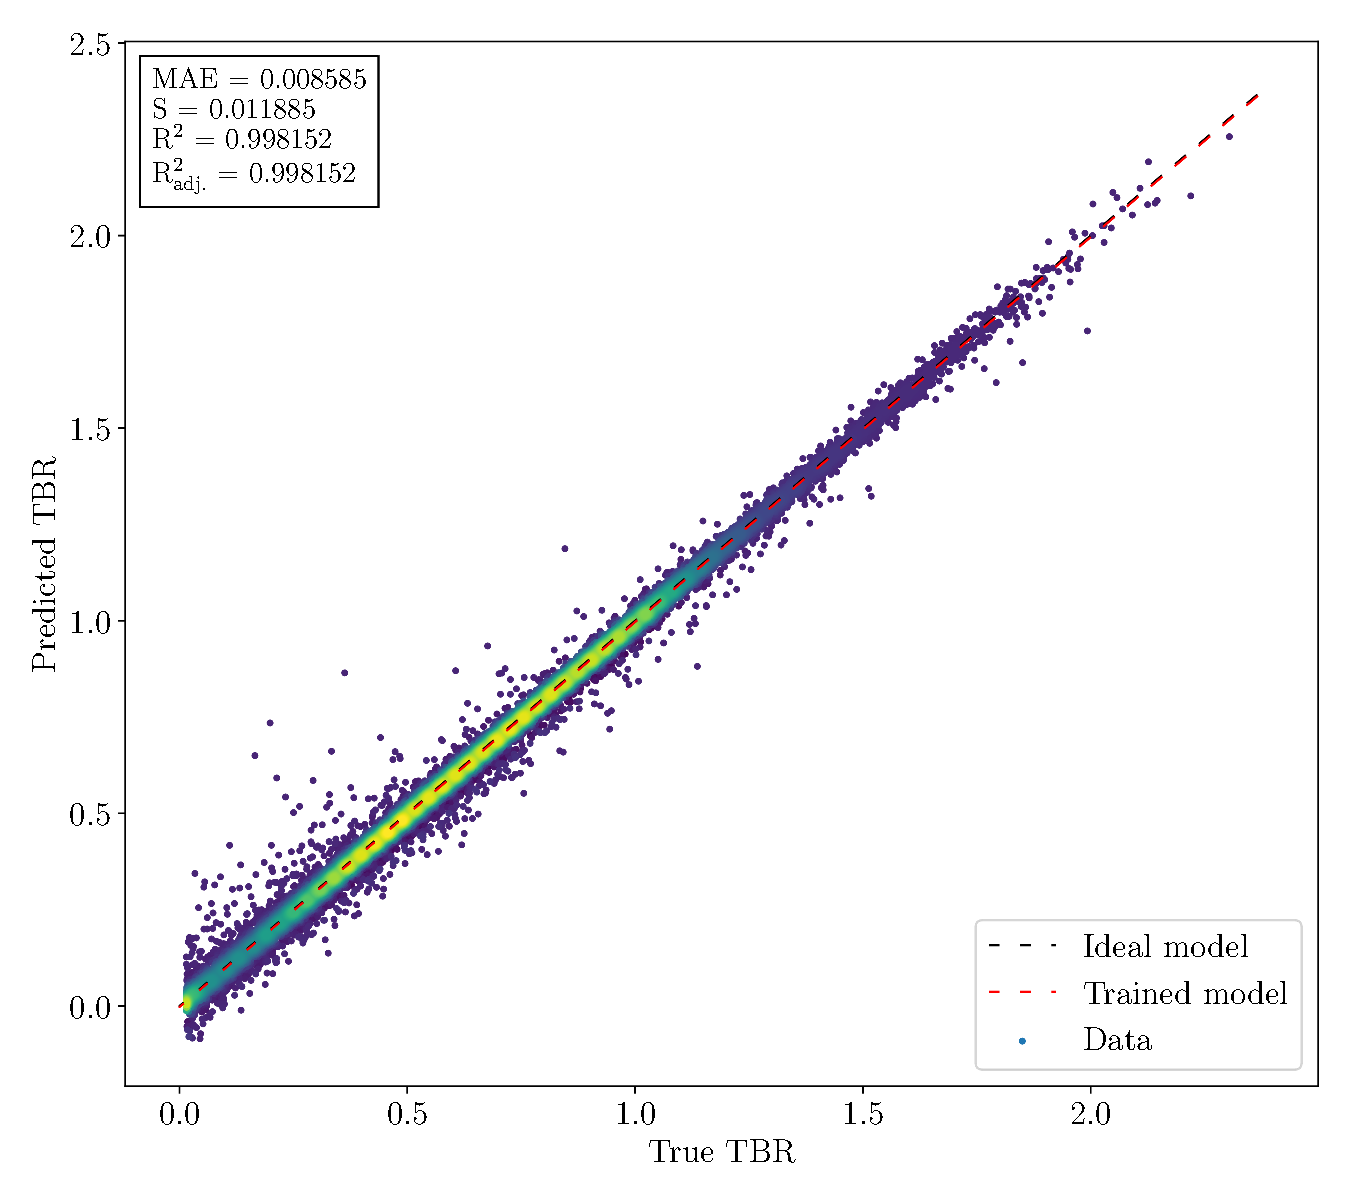
\includegraphics[height=83pt]{exp4_model6_rasterized}\vspace{-8pt}\\
		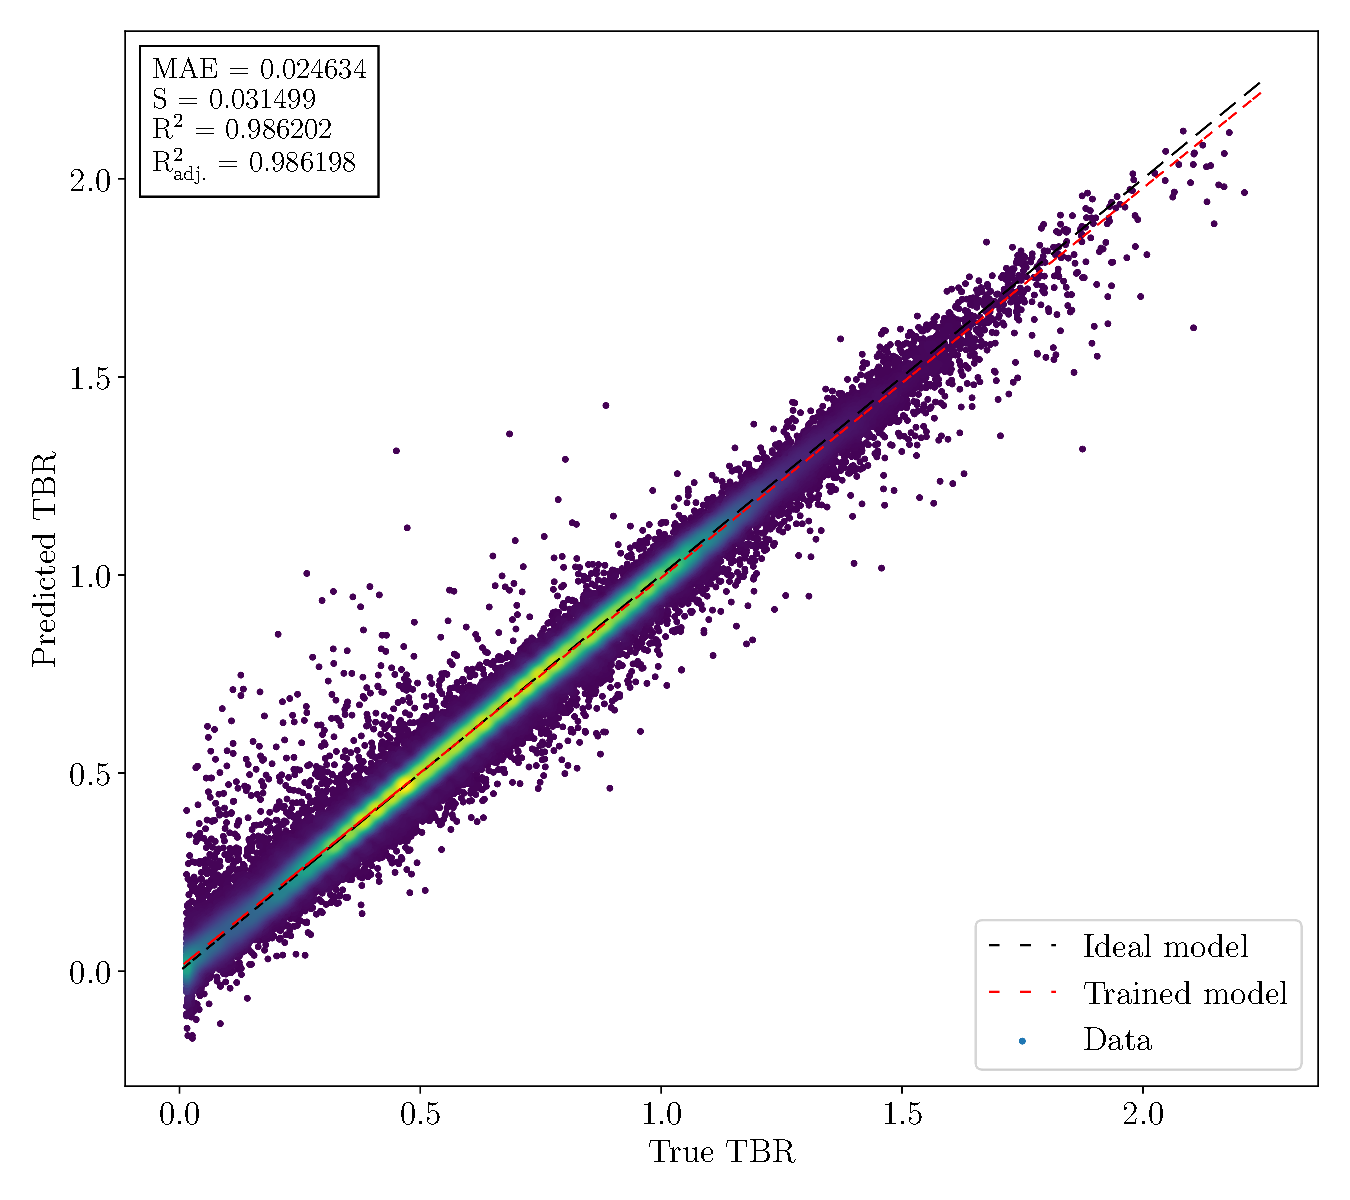
\includegraphics[height=83pt]{exp4_model7_rasterized}\vspace{-8pt}\\
		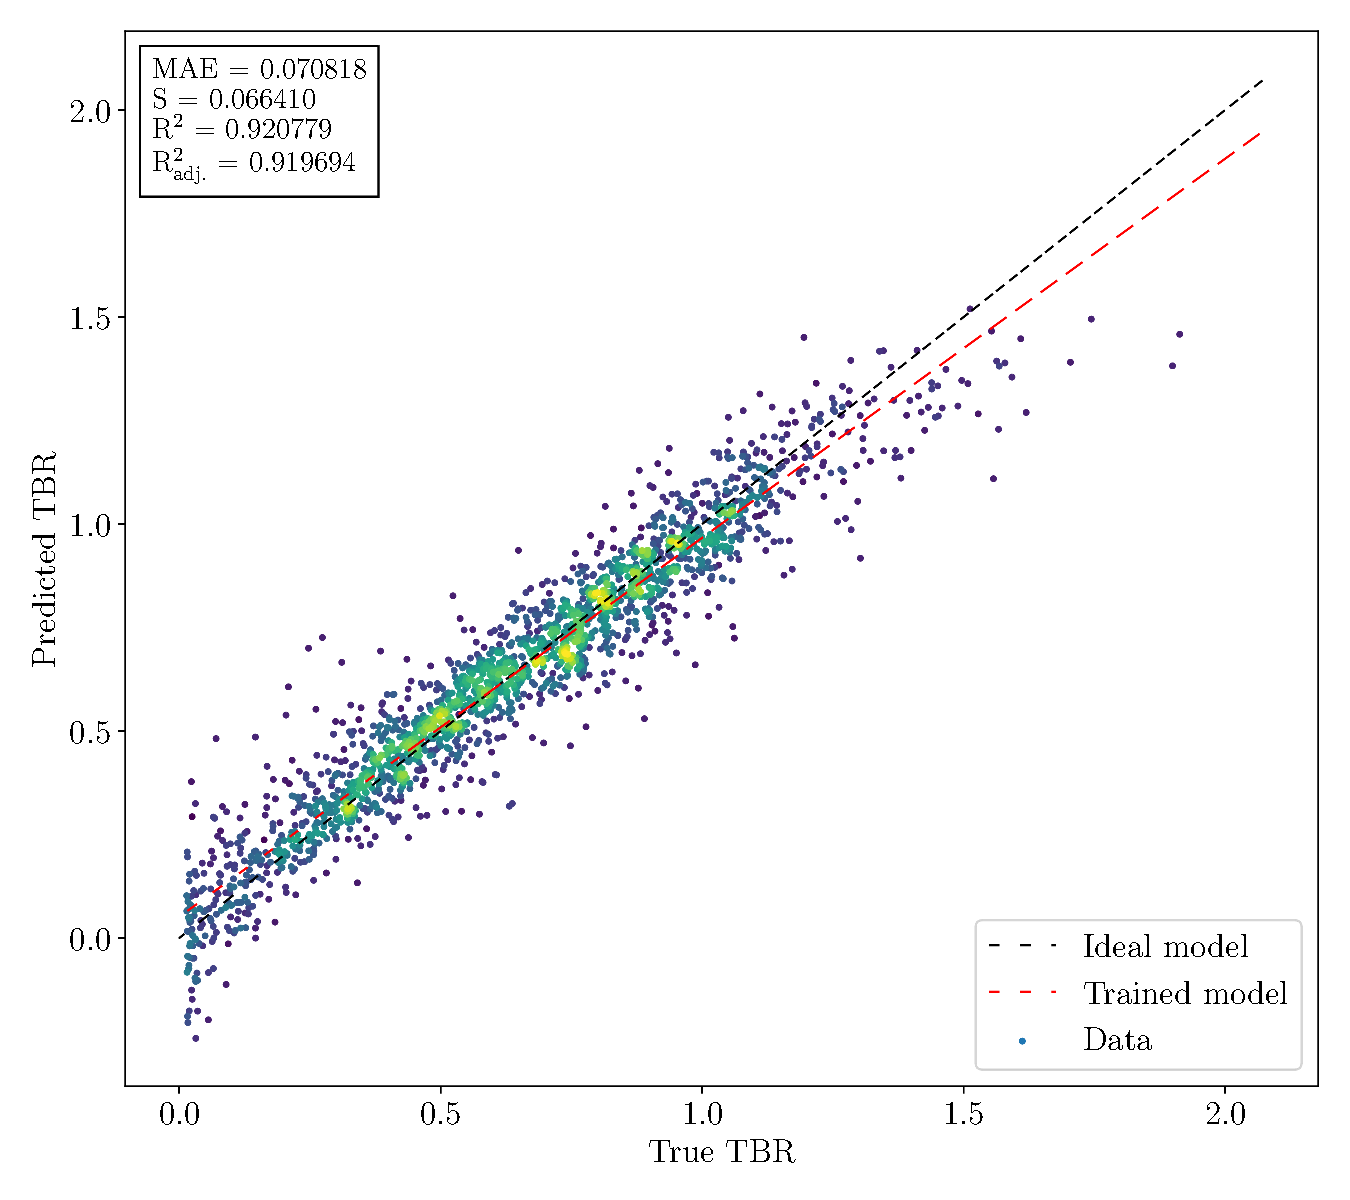
\includegraphics[height=83pt]{exp4_model3_rasterized}
	\end{columns}
\end{frame}
